\section{Introduction}
\label{sec:introdction}
Data exploration has gained lots of attentions over the last few years. The
main challenge is to support users with no clear requirements. To solve it,
several authors have proposed systems to ``play'' with the
data~\cite{abouzied2012dataplay, sellam2013meet, liarou2014dbtouch,
dimitriadou2014explore}. Typically, these systems propose some graphical
interface through which users can create, visualize and modify selections of
tuples quickly. Thus, users are engaged in a tight trial-and-error loop,
through which they discover their datasets.\\
These approaches are designed to help discovery. And indeed, they assume little
about the user's preliminary knowledge of the data. Yet, they rely on a crucial
assumption: they suppose that if a user sees an interesting set of tuples
(e.g., through tables or visualizations), they will recognize it immediately,
and think ``aha, this is interesting''. This assumption may hold with small
datasets, but it breaks down in higher dimensions. The first bottleneck is the
time necessary to inspect each column on after the other. The second one  is
humans' perception of high dimension spaces:  we cannot reasonably expect a
user to grasp more than three, maybe four dimensions. 

To cope with this problem, we suggest that the exploration system
\emph{describes} the tuples, in a language that users can understand. This
leads us to our problem statements:
\begin{framed}
    \everypar={{\setbox0=\lastbox}\everypar{}}
How can we describe a given set of tuples with natural language?
\end{framed}
In this paper, we introduce our algorithm, Ziggy. Ziggy's approach is to detect
subspaces for which the selected tuples are ``special'', i.e., have an unusual
distribution compared to the rest of the database. Then, for each of these
subspaces, it generates a natural language description of their distribution,
using statistical tests and hand-crafted rules. Here is an example of
description:
\begin{quote}
    Take a look at columns X, Y and Z. On X, and Y, your selection has a very
    low value. On column Z, your selection has a fairly low value, with high
    concentration. The correlation between Y and Z is unusually strong.\\
    You can also take a look at columns T. On this column, the
    values ``xxx'', ``yyy'', and ``ttt'' are underrepresented, while the values
    ``aa'' and ``bb'' are overrepresented.
\end{quote}

Several authors have tackled similar problems in the
past~\cite{angiulli2009detecting, knorr1999finding, loekito2008mining,
webb2008detecting}. None of them use natural language.

Our paper is built as follows. First, we discuss how to detect database views
in which a given set of tuple is ``special''. We expose the problem in its
generality, and discuss its relation to other methods, such as feature
selection. Second, we instantiate our problem with a custom objective function,
designed to yield interpretable results. Our function aggregates several
well-known statistical tests, carried out in a systematic, purposely
brute-force way.  Finally, we discuss how to describe the views with natural
language, and how to check the robustness of our results.

\section{General Problem Formulation}
\label{sec:problem}

\begin{figure}
  \centering
  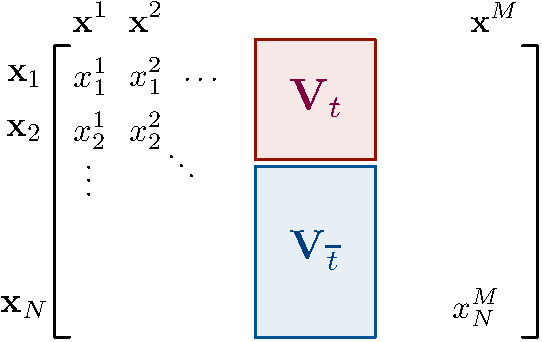
\includegraphics[width=0.6\columnwidth]{Figures/Notations}
  \caption{Notations.}
  \label{pic:notations}
\end{figure}
Let the matrix $\rb{D}$ with $M$ columns and $N$ rows represent our database.
We suppose that each tuple $\rb{x}_n = (x^1_n, \dots, x^M_n)^\top$ in the
database is an iid. sample from some unknown distribution
$p(\rb{x}_n)=p(\rb{x})$. We represent each column with a vector $\rb{x}^{m}=
(x^m_1, \dots, x^m_N)^\top$.  The user specifies a ``special'' selection of
tuples, described by the vector $\rb{t} = (t_1, \ldots, t_n)^\top$: $t_i=1$ if
the tuple is chosen, 0 otherwise. We refer to the tuples in the selection as
${\rb{D}}_t$, and the remaining tuples as ${\rb{D}}_{\overline{t}}$. We refer
to the underlying distributions as $p(\rb{x}|t)$ and $p(\rb{x}|\overline{t})$
respectively. We illustrate these notations with Figure~\ref{pic:notations}.

Our model is based on a user-specified \textbf{mass dissimilarity measure}
$\mf{D}(\rb{D}, \rb{D}')$, which measures the difference between two groups of
tuples. If the rows of $\rb{D}$ and $\rb{D}'$ are sampled from the same
distribution $p(\rb{x}) = p'(\rb{x}')$, then $\mf{D}$ is very close to 0. If
not, $\mf{D}$ grows with the dissimilarity of the distributions.
Figure~\ref{pic:sameMean} gives an example of the latter case.  Here are some
possible choices:
\begin{itemize}
    \item The hypothesis testing literature provides lots of examples. For
        instance, if $\rb{\mu}$ and $\rb{\mu}'$ represent the averages of $\rb{D}$ and
        $\rb{D'}$, and if $\rb{S}$ is an estimate of their pooled covariance
        matrix, we can set $\mf{D}(\rb{D}, \rb{D}') \equiv (\rb{\mu} -
        \rb{\mu'})^\top \rb{S}^{-1} ( \rb{\mu} -
        \rb{\mu'})$. The advantage of this approach is that we know the
        asymptotic distribution of $\mf{D}(\rb{D}, \rb{D}')$, and thus we can
        easily test its significance.
    \item A more general option is to estimate the Kullback-Leibler divergence:
        $\mf{D}(\rb{D}, \rb{D}') \equiv KL(\hat{p}(\rb{x});
        \hat{p}'(\rb{x}'))$, where $\hat{p}(\rb{x})$ and $\hat{p}'(\rb{x}')$
        are density estimators. This approach can cope with both continuous and
        categorical variables, and it has firm theoretical foundations.
    \item With the same notations, an other approach is to define:
        $\mf{D}(\rb{D}, \rb{D}') \equiv 1 -  \hat{p}(\rb{D}') \cdot
        \hat{p'}(\rb{D})$. This measure is also general, and it is normalized
        (it varies between 0 and 1).
\end{itemize}
Knowing this function $\mf{D}$, we can already propose a first, naive,
formulation of our problem. We want to find groups of variables for which the
distribution of the chosen tuples is different from that of the rest of the
data.
\begin{problem}
    Consider a distribution dissimilarity function $\mf{D}$ and two integers
    $K$ and $D$. Find the top $K$ distinct views $\rb{D}^i = [\rb{x}^1, \dots,
    \rb{x}^d]$ with at most $D$ dimensions which maximize: $ \mf{D}\big(
    \rb{D}^i_t ; \rb{D}^i_{\overline{t}} \big)$ (ignoring column permutations).
\end{problem}
\begin{figure}
  \centering
  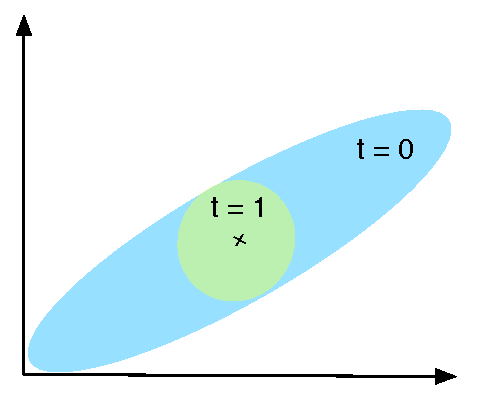
\includegraphics[width=0.8\columnwidth]{Figures/SameMean}
  \caption{Example of interesting view.}
  \label{pic:sameMean}
\end{figure}
This approach is simple, but it can lead to lots of redundancy: a small number
of good columns may dominate the results and appear in all $K$ views. In a data
exploration scenario, users may value \emph{diversity}, even if the views are
sub-optimal. To enforce this requirement, we introduce a penalty factor in our
objective function.

To measure redundancy, we need a \textbf{dependency measure} $\mf{S}$, which
measures the statistical dependency between the underlying distributions of two
sets of tuples $\rb{D}$ and $\rb{D}'$.  Here are some possible choices:
\begin{itemize}
    \item We can use a simple linear coefficient, or a its multivariate
        generalization, the RV-coefficient.
    \item Alternatively, we can estimate the mutual information of the
        underlying variables:
        $\mf{S}(\rb{D}', \rb{D}') \equiv \hat{I}(\rb{x}, \rb{x'})$.
\end{itemize}
We can now introduce a new version of our problem. We seek views
which maximize the distance statistic, while minimizing inter-view dependency.
We define this problem in a recursive way:
\begin{problem}
    Suppose that we have already detected $i$ views. We obtain $\rb{D}^{1..i} =
    [\rb{D}^1, \ldots, \rb{D}^i]$ by concatenating these views.  Given a
    positive real $\lambda$, find the view $\rb{D}^{i+1}$ with at most $D$
    columns which maximizes:
        \begin{equation}
            \label{prob1}
            \mf{D}\big( \rb{D}^{i+1}_t  ; \rb{D}^{i+1}_{\overline{t}} \big) - 
            \lambda \cdot \mf{S} ( \rb{D}^{i+1} ; \rb{D}^{1..i})
        \end{equation}
\end{problem}
Observe that the parameter $\lambda$ controls the trade-off between mass distance
and view diversity. For some $L$, an equivalent way to express our problem is
the following:
\begin{equation}
    \label{prob2}
    \begin{aligned}
        & \text{Argmax}_{\rb{D}^{i+1}} 
            & \mf{D}\big( \rb{D}^{i+1}_t  ; \rb{D}^{i+1}_{\overline{t}} \big)\\
        & \text{s.t.} 
        &\mf{S} ( \rb{D}^{i+1} ; \rb{D}^{1..i}) & < L\\ 
    \end{aligned}
\end{equation}
Equation~\ref{prob1} in the Lagrangian of Equation~\ref{prob2}, up to an
additive constant.

At this point, we notice that our problem is very to close to \emph{feature
selection}. Feature selection seeks columns of $\rb{D}$ from which we can
predict $\rb{t}$. Ultimately, the goal is to estimate $p(t|\rb{x})$. Our
problem is symmetric: we seek columns of $\rb{D}$ which \emph{are predicted} by
$\rb{t}$.  Hence, we focus on $p(\rb{x}|t)$. According to Bayes' theorem, these
two problems are equivalent. And indeed, some feature selection methods, such
as LDA, are also based on $p(\rb{x}|t)$.

The differences do not stop here. Recall that Ziggy focuses on
\emph{interpretation}, while feature selection algorithms focus on
\emph{prediction}. Therefore, Ziggy returns a few, non-redundant views, while
classic algorithms focus on single, potentially complex views. Also, most
feature selection algorithms optimize \emph{class separability}. In this paper,
we are interested in \emph{any} kind of dissimilarity. For instance, most
feature selection algorithms would reject the view presented
in Figure~\ref{pic:sameMean}. For Ziggy, this view is perfectly acceptable. 

Finally, we may wonder what is the difference between Ziggy and Claude. After
all, they are quite similar. I discuss this point in the Appendix.


\section{Instantiation: Meet Ziggy}
\label{sec:instantiation}

\subsection{Explainable Mass Dissimilarity}
\label{sec:explain}

We now discuss how to instantiate the function~$\mf{D}$. In principle, we could
borrow a very general divergence measure from the statistics literature, such
as the KL-divergence.  Such instantiation, coupled with visualization
technology, would be perfectly suited to a expert user. Instead, we chose to
focus on non-experts. We introduce the \textbf{Z-dissimilarity} (Ziggy's
Dissimilarity), an admittedly naive, but \emph{explainable} mass dissimilarity
measure.

To obtain the Z-dissimilarity between two sets of tuples, we operate as
follows. First, we compute several univariate dissimilarity indicators $z^1,
\ldots, z^Z$.  Each of them highlights a specific difference between $\rb{D}_t$
and $\rb{D}_{\overline{t}}$, based on one-dimension statistics. For instance,
they describe the difference between means, or the ratio of the variances, for
each variable $\rb{x}^m$ separately.  We call them \textbf{z-dissimilarities}
(notice the lower-cased z). In a second step, we compute bivariate
z-dissimilarities. They describe possible differences with regards to
dependency: for instance, the regression line between two variables may be
steeper for our special tuples. Finally, we concatenate all these scores in a
vector $\rb{z}=(z^1_1, \ldots, z^Z_M)$, and aggregate them using the norm
$\norm{\rb{z}}_P=\left(\sum_{z \in \rb{z}} w_z \cdot |z|^P \right)^{1/P}$, with
optional weights $w_z$.

\textbf{[Maybe there are smarter ways to aggregate the statistics, using e.g.,
multiple testing. To be looked into.]}

\begin{table}[t!]
    \centering
    \begin{tabular}{|c|c|c|c|}
      \hline
      Property & Type 1 & Type 2 & z-dissimilarity \\
      \hline
      Mean        & Contin.  & - & T-test\\
      Variance    & Contin.  & - & F-test\\
      Frequencies & Discrete & - & Chi-square\\
      \hline
      Dependence  & Contin. & Contin & Dif. Correlation\\
      Dependence  & Contin. & Discrete & Dif. Kom.-Smir.\\
      Dependence  & Discrete & Discrete & Dif. Chi-square \\
      \hline
    \end{tabular}
\caption{Our choice of z-dissimilarites for different data types. In the
bivariate case we actually compute statistics of statistics.}
    \label{tab:dissim}
\end{table}

How should we chose our z-dissimilarites? Each indicator should describe an
interpretable property of the data. Also, for meaningful results, the
dissimilarities should be normalized. We selected a battery of well-known test
statistics from the literature, described in Table~\ref{tab:dissim}. In the
univariate case, we use these test without any modification. In the bivariate
case, we derive \emph{statistics of statistics}. Consider for instance a pair
of continuous variables. We are not interested in the correlation between these
columns as such. Instead, we are interested in its variation when we replace
$\rb{D}_{t}$ by $\rb{D}_{\overline{t}}$. Hence, the z-dissimilarity reports the
\emph{difference} between the correlations, not the correlations themselves. We can
obtain the asymptotic distribution of this statistic analytically.
[\textbf{or at least I hope so}]

Observe that we compute univariate, then bivariate statistics. In principle, we
could test spaces with more dimensions. We chose not to do so, for two
practical reasons. First, we suppose that relationships in three
dimensions or more are harder to convey and understand in natural language.
Second, the number of relationships to be tested grows exponentially with the
dimensionality of the test (up to tests of dimension $M/2$). This harms Ziggy's
runtime, and it leads to much longer explanations.


\subsection{Dependency Measure}
\label{sec:dependency}

We now discuss how to instantiate the dependency measure~$\mf{S}$. As discussed
in Section~\ref{sec:problem}, we face a large choice. Our recommendations
depend on the computing resources available. If those are plentiful, we suggest
to use a general dependency measure such as the Mutual Information. The
advantage of this option is that it captures both linear and non-linear
relationships. Under scarcity, we suggest to use a measure based on the linear
correlation. We prefer this approach because it reuses intermediate results necessary to
compute the Z-distance: we obtain the pairwise correlations ``for free''.


\section{Model Validation}
\label{sec:validation}

We now focus on the following problem: how \emph{significant} are the
dissimilarities associated to our views? Let us consider the general
case. We want to test a view $\rb{D}$, with mass dissimilarity $d = \mf{D}(
\rb{D}_t  ; \rb{D}_{\overline{t}})$. A high value may indicate that  $\rb{D}_t$
and $\rb{D}_{\overline{t}}$ come from two different distributions. But it could
also be caused by chance. How confident are we of this result? Note that this
section deals with the \emph{aggregated} dissimilarity: in Ziggy's case, this
means that we want to test the Z-dissimilarity, not the individual
z-dissimilarities (in fact, we already know their significance).

The statistics literature provides us a completely generic way to solve this
problem: permutation testing. The idea is to shuffle the rows of $D$, without
modifying $\rb{t}$. Thus, the tuples are randomly affected to $\rb{D}_t$ and
$\rb{D}_{\overline{t}}$. We then measure the new distance $d=\mf{D}\big(
\rb{D}^{i+1}_t  ; \rb{D}^{i+1}_{\overline{t}} \big)$. We repeat the experiment
$B$ times, and obtain the results $d^1, \ldots, d^B$. We compare them to our
initial measurement $d$. If $p\%$ samples are greater than $d^0$, then our
p-value is approximately $p$.

\textbf{[Problem: how can we quickly reshuffle the rows of
$\rb{D}$? Maybe a fast solution is to use random hash functions. To be
looked into, there may be a nice secondary contribution there!]}




\section{Experiments}
\label{sec:experiments}

\section{Conclusion}
\label{sec:conclusions}
